\documentclass[10pt]{beamer}
\usetheme{jambro}

\title[]{Microeconomia I - Apresentação}
\author[]{Paulo Victor da Fonseca}
\date{28 de fevereiro de 2023}

\hypersetup{
    colorlinks = true,
    urlcolor = teal,
    linkcolor = white    
}
\usepackage[portuguese]{babel}
\usepackage{subfig}
\usepackage{emoji}

\begin{document}

\begin{frame}[plain]
    \titlepage{
        \begin{center}
            \begin{minipage}{0.8\textwidth}
                \centering
            \end{minipage}
        \end{center}}
\end{frame}

\section{Docente}
\begin{frame}{Docente}
    \begin{tabular}{cl}
        \begin{tabular}{c}
            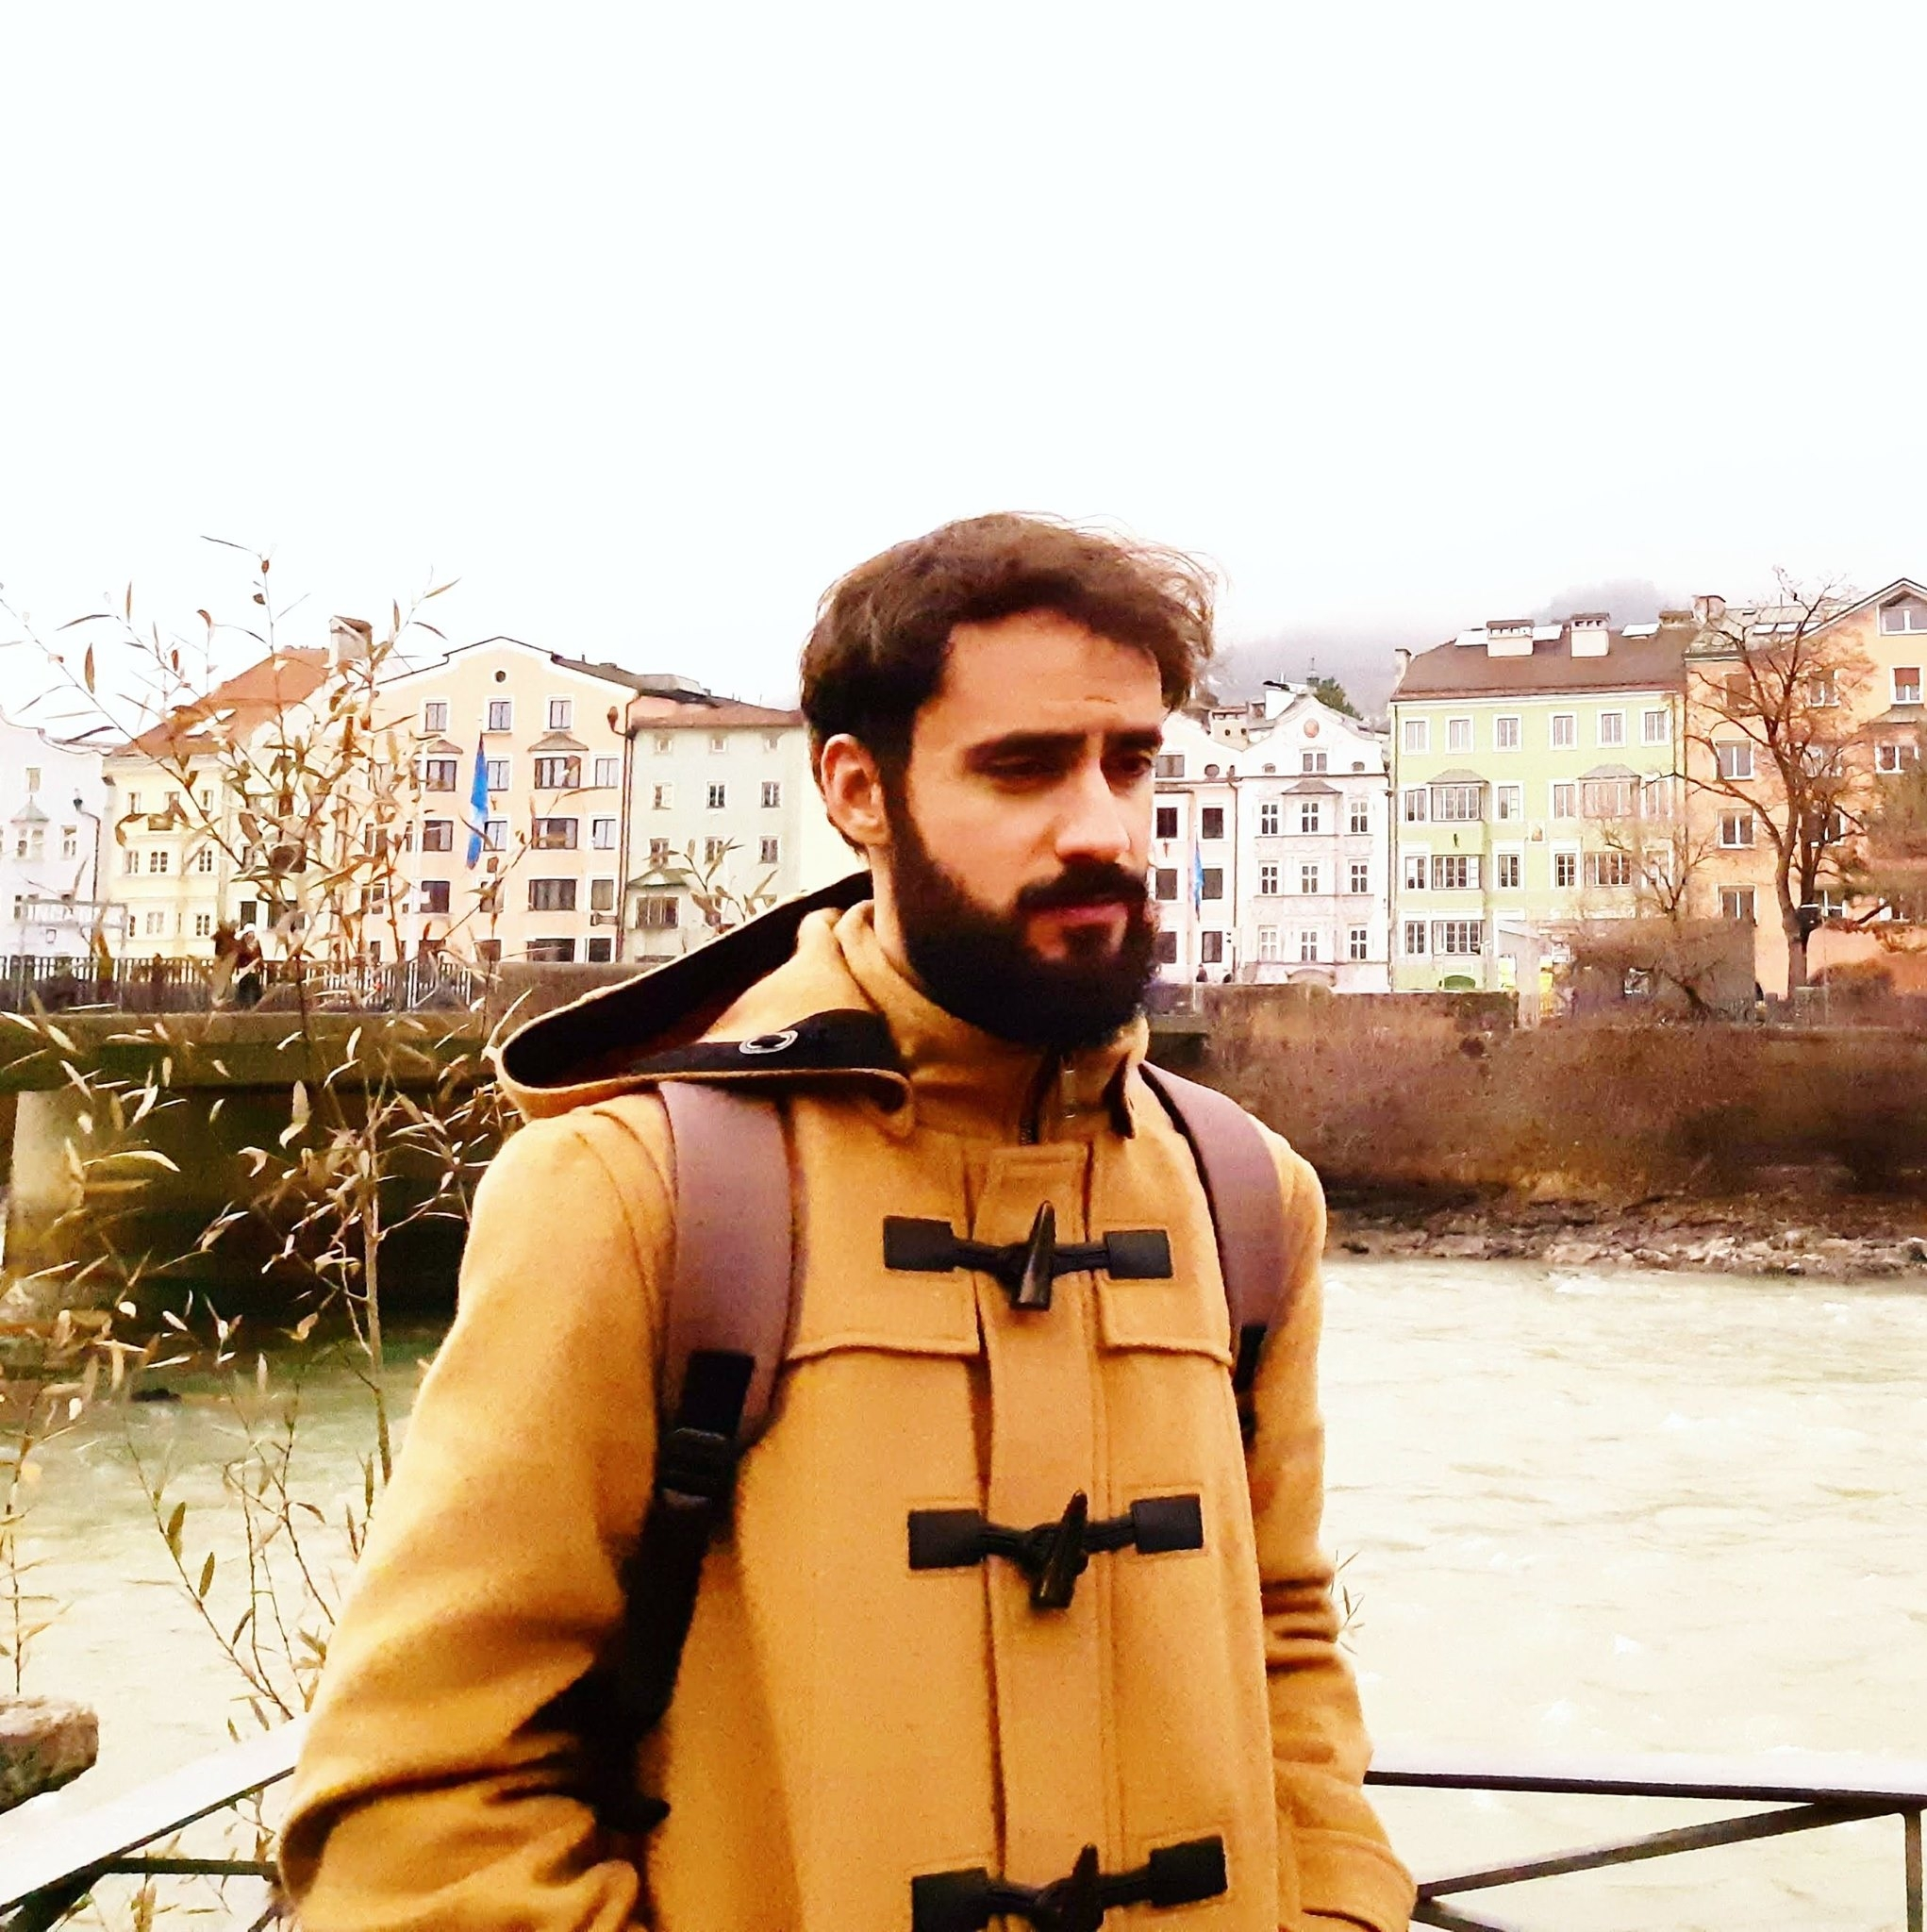
\includegraphics[width=3.5cm]{./figures/Paulo}
        \end{tabular}
         & \begin{tabular}{l}
               \parbox{0.6\linewidth}{
                   \begin{itemize}
                    \item \textbf{Nome:} Paulo Victor da Fonseca\medskip
                    \item \textbf{Formação:} Doutorado em Economia - UFSC\medskip
                    \item \textbf{Áreas de pesquisa:} Macroeconomia. Políticas monetária e fiscal. Modelos DSGE. Modelos novo-Keynesianos com agentes heterogêneos. Modelos baseados em agentes.\medskip
                    \item \textbf{Website:} \href{https://pvfonseca.github.io}{pvfonseca.github.io}\medskip
                    \item \textbf{Contato:} \href{mailto:paulo.fonseca@udesc.br}{paulo.fonseca@udesc.br}
                \end{itemize}
               }
           \end{tabular} \\
    \end{tabular}
\end{frame}

\section{Motivação}
\begin{frame}{Microeconomia I}
    \begin{tabular}{cl}
        \begin{tabular}{l}
            \parbox{0.6\linewidth}{
                \NB{A economia \'{e} um estudo da humanidade na atividade comum da vida. \\ \medskip \href{https://pt.wikipedia.org/wiki/Alfred_Marshall}{Alfred Marshall, Princípios de Economia (1890)}}
            }
        \end{tabular}
        & \begin{tabular}{c}
            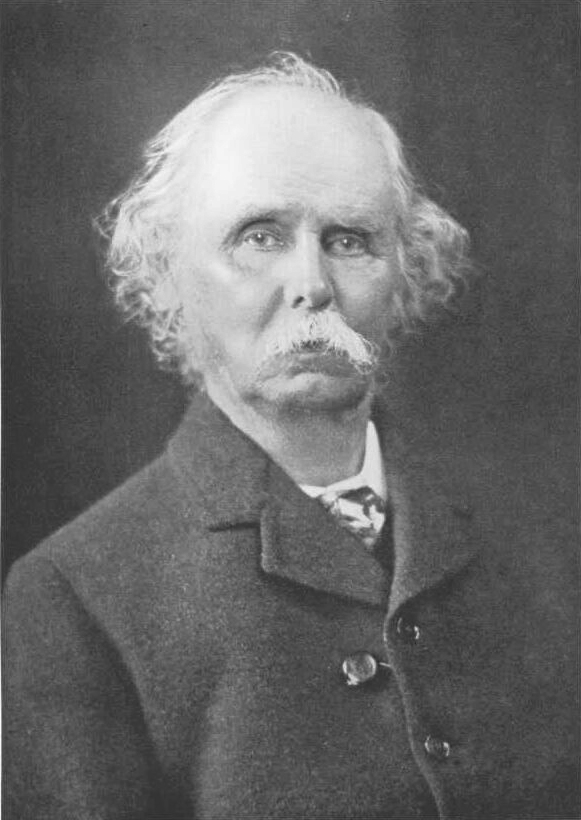
\includegraphics[width=3.5cm]{./figures/marshall.jpg}
        \end{tabular}  \\
    \end{tabular}
\end{frame}

\begin{frame}{Microeconomia I}
    \begin{itemize}
        \item \hlight{Economia \'{e} o estudo da aloca\c{c}\~{a}o de recursos escassos.}\bigskip
        \item Recursos escassos e demandas quase ilimitadas: estabelecer critérios para decidir quantos e quais bens e serviços serão produzidos, e como serão alocados entre agentes. \bigskip
        \item Para determinar alocação ótima de recursos, é necessário estudar o comportamento dos agentes no ambiente econômico.
    \end{itemize}
\end{frame}

\begin{frame}{Microeconomia I}
    \begin{itemize}
        \item A economia divide-se em dois ramos principais: microeconomia e macroeconomia. \bigskip

        \item A \tikz[tstyle]{\node[nstyle](node2){microeconomia}} trata do comportamento das unidades (agentes) econômicas individuais. \bigskip
              \begin{tikzpicture}[tpstyle]
                  \draw[pencil,very thick] ([yshift=-2pt]node2.south west) to ([yshift=-2pt]node2.south east);
              \end{tikzpicture}

        \item Neste curso, focaremos em dois tipos de agentes econômicos: \medskip
        \begin{enumerate}
            \item \hlight{Consumidores}: manifestam ações por intermédio de suas demandas.\medskip
            \item \hlight{Firmas}: manifestam suas ações por intermédio de suas demandas por insumos ou fatores de produção e por sua oferta de bens e serviços produzidos.
        \end{enumerate}
    \end{itemize}
\end{frame}

\begin{frame}
    {Microeconomia I}
    \begin{itemize}
        \item Ofertas e demandas dos agentes são representadas no mercado. \bigskip
        \item Quantidades demandadas e ofertadas por cada agente dependem, portanto, dos preços dos bens e dos insumos.\bigskip
        \item Mercado: cotação de preços e verifica as quantidades demandadas e ofertadas a cada nível possível de preço.\bigskip
        \item Se quantidade ofertada = quantidade demandada, dizemos que o mercado está em equilíbrio.\bigskip
        \item Existem vários mercados em um sistema econômico. Pelo menos um para cada bem ou serviço existente.
    \end{itemize}
\end{frame}

\begin{frame}
    {Microeconomia I}
    \begin{itemize}
        \item Dada a complexidade do sistema econômico, economistas utilizam \tikz[tstyle]{\node[nstyle](node0){modelos econômicos}}.\bigskip
        \begin{tikzpicture}[tpstyle]
            \draw[pencil, very thick] ([yshift=-2pt]node0.south west) to ([yshift=-2pt]node0.south east);
        \end{tikzpicture}
        \item Modelos devem abstrair de grande parte das complexidades e focar apenas nos elementos essenciais à análise em questão.\bigskip
        \item Apesar de abstrações, modelos fornecem auxílio fundamental para o entendimento do comportamento econômico.        
    \end{itemize}
\end{frame}

\begin{frame}
    {Microeconomia I}
    \begin{tabular}{cl}
        \begin{tabular}{c}
            \href{https://en.wikipedia.org/wiki/Essays_in_Positive_Economics}{
\includegraphics[width=3.5cm]{./figures/EssaysInPositiveEconomics.jpg}} \\
            \tiny{{\scshape Friedman, M.} Essays in positive economics (1953).}
        \end{tabular}
         & \begin{tabular}{l}
               \parbox{0.6\linewidth}{
                \begin{itemize}
                    \item Métodos para validação de modelos econômicos teóricos:\medskip
                    \begin{enumerate}
                        \item \tikz[tstyle]{\node[nstyle](node0){Abordagem direta}}: busca validar os pressupostos básicos nos quais um modelo é baseado.\medskip
                        \item \tikz[tstyle]{\node[nstyle](node1){Abordagem indireta}}: busca confirmar a validade ao mostrar que um modelo simplificado corretamente prediz eventos do mundo real.\medskip
                    \end{enumerate}
                    \item Exemplo: modelo de maximização de lucros.
                \end{itemize}
               }
           \end{tabular} \\
    \end{tabular}    
        \begin{tikzpicture}[tpstyle]
            \draw[pencil, very thick] ([yshift=-2pt]node0.south west) to ([yshift=-2pt]node0.south east);
            \draw[pencil, very thick, brick] ([yshift=-2pt]node1.south west) to ([yshift=-2pt]node1.south east);
        \end{tikzpicture}    
\end{frame}

\begin{frame}{Microeconomia I}
    \begin{itemize}
        \item \hlight{Caracter\'{i}sticas gerais} - Apesar da enorme variedade de modelos econômicos, praticamente todos incorporam 3 elementos comuns:\medskip
        \begin{itemize}
            \item Hipótese de \emph{ceteris paribus}\medskip
            \NB{\emoji{warning} \small{Alguns fatores são invariantes durante o período de análise $\Rightarrow$ Dificuldades para verificação empírica de modelos dada inabilidade de conduzir experimentos controlados ($\neq$ ciências físicas).}}\medskip
            \item Agentes otimizadores\medskip
            \item Distinção cuidadosa entre questões normativas e positivas\bigskip
        \end{itemize}        
    \end{itemize}
\end{frame}

\begin{frame}{Microeconomia I}
    \begin{itemize}
        \item Modelos que estudaremos possuem estrutura matemática e evidenciam as relações entre fatores que afetam decisões dos agentes e os resultados destas decisões.\bigskip
        \begin{itemize}
            \item \tikz[tstyle]{\node[nstyle](node0){Variáveis exógenas:}} fatores que estão fora do controle do tomador de decisão \medskip
            \item \tikz[tstyle]{\node[nstyle](node1){Variáveis endógenas:}} variáveis determinadas dentro do modelo
        \end{itemize}
        \begin{tikzpicture}[tpstyle]
            \draw[pencil, very thick] ([yshift=-2pt]node0.south west) to ([yshift=-2pt]node0.south east);
            \draw[pencil, very thick, blue] ([yshift=-2pt]node1.south west) to ([yshift=-2pt]node1.south east);
        \end{tikzpicture}    
    \end{itemize}
\end{frame}

\begin{frame}{Microeconomia I}
    \begin{center}
		\begin{tikzpicture}
			% HOME
			%--------------
			% Home Banks
			\node[fill=title!70,text=white,rounded corners,inner sep=1ex,font=\bfseries,xshift=0cm,yshift=3cm] (Exo) {Variáveis Exógenas};
			% Home Firm
			\node[fill=title!70,text=white,rounded corners,inner sep=1ex,font=\bfseries,xshift=0cm,yshift=0cm] (Model) {Modelo Econômico};
			% Home Households
			\node[fill=title!70,text=white,rounded corners,inner sep=1ex,font=\bfseries,xshift=0cm,yshift=-3cm] (Endo) {Variáveis Endógenas};
			% Arrows 
			\draw[snake,black,->,very thick] ([xshift=-0cm]Exo.west) to [bend right] ([yshift=-0cm]Model.west);
            \draw[snake,black,->,very thick] ([xshift=-0cm]Exo.east) to [bend left] ([yshift=-0cm]Model.east);
			\draw[arrow,black,->,very thick] ([xshift=-0cm]Model.west) to [bend right] ([yshift=-0cm]Endo.west);
            \draw[arrow,black,->,very thick] ([xshift=-0cm]Model.east) to [bend left] ([yshift=-0cm]Endo.east);
			% Firmas
			\draw[] (3.6cm,1.75cm) node[anchor=north,opacity=1,] {\small \hand \footnotesize{Preços de insumos}};
            \draw[] (3.5cm,1.5cm) node[anchor=north,opacity=1,] {\small \hand \footnotesize{e mercadorias}};
			\draw[title!70] (3.5cm,2.7cm) node[anchor=north,opacity=1,] {\small \hand FIRMAS};
            \draw[] (3.6cm,0.3cm) node[anchor=north,opacity=1,] {\small \hand \footnotesize{Maximização de lucro}};
            \draw[] (3.6cm,-1.3cm) node[anchor=north,opacity=1,] {\small \hand \footnotesize{Qtdade produzida}};
            \draw[] (3.6cm,-1.5cm) node[anchor=north,opacity=1,] {\small \hand \footnotesize{Insumos contratados}};
            % Consumidores
			\draw[] (-3.8cm,1.75cm) node[anchor=north,opacity=1,] {\small \hand \footnotesize{Preços de mercadorias}};            
			\draw[title!70] (-4cm,2.7cm) node[anchor=north,opacity=1,] {\small \hand CONSUMIDORES};
            \draw[] (-3.8cm,0.3cm) node[anchor=north,opacity=1,] {\small \hand \footnotesize{Maximização de utilidade}};
            \draw[] (-3.6cm,-1.3cm) node[anchor=north,opacity=1,] {\small \hand \footnotesize{Qtdade demandada}};            			
		\end{tikzpicture}
	\end{center}
\end{frame}

\begin{frame}{Microeconomia I}
    \begin{itemize}
        \item Muitos dos modelos econômicos são estruturados a partir da hipótese de que os agentes buscam seus objetivos de maneira \hlight{racional}.\bigskip
        \NB{\emoji{warning} Racionalidade, em economia, não significa exclusão de comportamentos prejudiciais ao próprio indivíduo.}\bigskip
        \item A hipótese de racionalidade é amplamente aceita: \medskip
        \begin{itemize}
            \item Hipóteses de comportamento otimizador são úteis para gerar modelos precisos e solucionáveis \medskip
            \item Validação empírica aparente
        \end{itemize}
    \end{itemize}
\end{frame}

\begin{frame}{Microeconomia I}
    \begin{itemize}
        \item A análise econômica pode ser classificada como positiva ou normativa: \bigskip
        \begin{itemize}
            \item \tikz[tstyle]{\node[nstyle](node1){Análise econômica positiva:}} descrição e explicação dos fenômenos econômicos observáveis \medskip
            \item \tikz[tstyle]{\node[nstyle](node0){Análise econômica normativa:}} foca em proposições normativas (como o mundo "deveria" ser), envolve julgamentos de valor
        \end{itemize}
    \end{itemize}
    \begin{tikzpicture}[tpstyle]
        \draw[pencil, very thick] ([yshift=-2pt]node0.south west) to ([yshift=-2pt]node0.south east);
        \draw[pencil, very thick, blue] ([yshift=-2pt]node1.south west) to ([yshift=-2pt]node1.south east);
    \end{tikzpicture}
\end{frame}

\begin{frame}{Microeconomia I}
    \begin{itemize}
        \item Outro objeto de estudo: compreensão de como unidades econômicas interagem para formar unidades maiores - mercados e indústrias. \bigskip
        \item Com o estudo do comportamento e da interação entre cada empresa e consumidores, a micro revela como setores e mercados operam e se desenvolvem, por que são diferentes entre si e como são influenciados por políticas governamentais e condições econômicas globais.\bigskip

        \item Algumas questões que podem ser analisadas pelas ferramentas microeconômicas: \bigskip
        \begin{itemize}
            \item Aumento de um imposto qualquer \medskip
             \item Aumento da punição de certos tipos de crimes \medskip 
             \item Liberalização das drogas \medskip
             \item Discriminação racial, etc.
        \end{itemize}
    \end{itemize}
\end{frame}

\begin{frame}{Microeconomia I}
    \begin{itemize}
        \item \hlight{Economia de mercado:} sistema de preços opera livremente. \bigskip
        \item Sistema de preços é fundamental para alocação de recursos: informações e incentivos que coordenam a decisão de milhares de agentes. \bigskip
        \item Cada agente precisa conhecer apenas os preços dos produtos que afetam seu objetivo para tomar suas decisões. \bigskip
        \item \hlight{Economia descentralizada:} agentes decidem o que consumir ou produzir sem necessidade de um coordenador central.
    \end{itemize}
\end{frame}

\begin{frame}{Microeconomia I}
    \begin{tabular}{cl}
        \begin{tabular}{l}
               \parbox{0.6\linewidth}{
                \begin{itemize}
                    \item Apesar da falta aparente de coordenação, mercado de \hlight{competição perfeita} é eficiente economicamente: \tikz[tstyle]{\node[nstyle](node0){mão invisível}}\medskip
                    \begin{enumerate}
                        \item \tikz[tstyle]{\node[nstyle](node1){Economia centralizada}} - planejador central precisa conhecer preferências e tecnologias $\times$ \tikz[tstyle]{\node[nstyle](node2){economia descentralizada}} - economia de informação. \medskip
                        \item Consumidores - desejam pagar menor preço possível, firmas - vender pelo preço mais alto. Na economia de mercado, bens são produzidor por firmas mais eficientes e consumidos por consumidores que atribuem maior valor aos bens.
                    \end{enumerate}
                \end{itemize}
               }               
           \end{tabular}
           & \begin{tabular}{c}
            \href{https://pt.wikipedia.org/wiki/Adam_Smith}{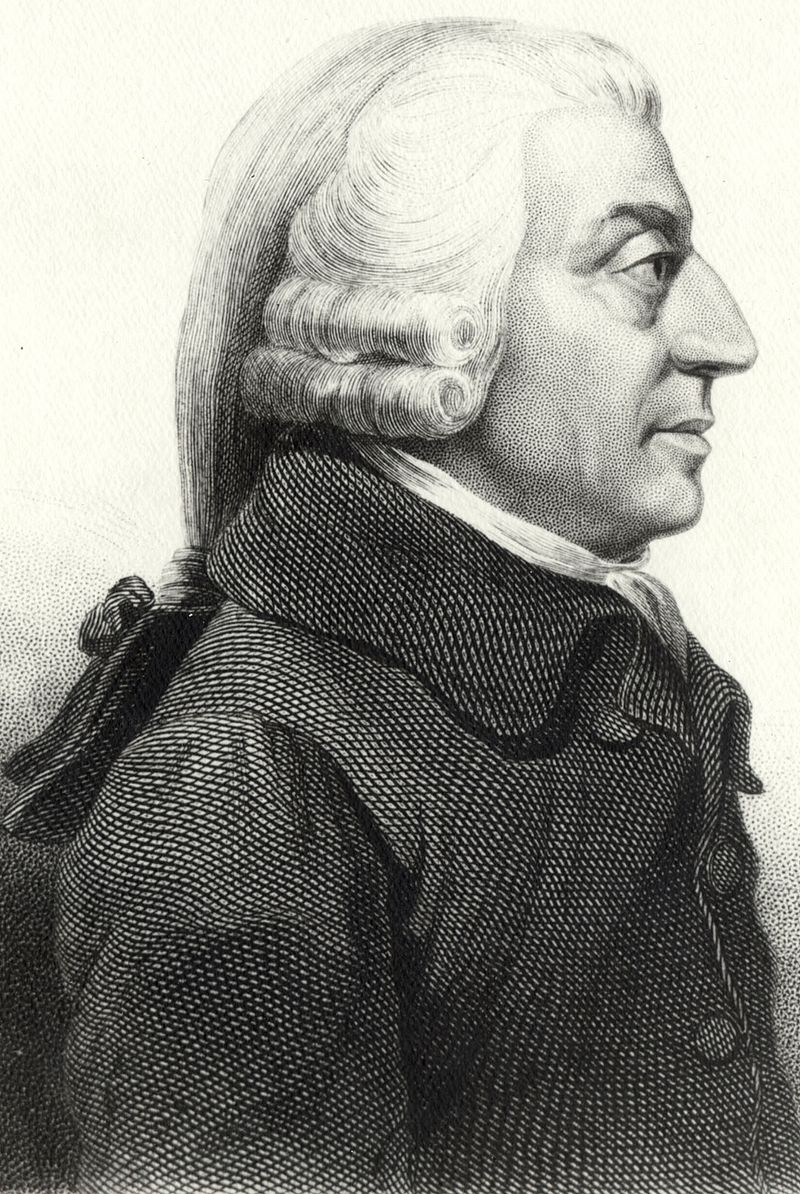
\includegraphics[width=3.5cm]{./figures/smith.jpg}} \\
            \tiny{{\scshape Adam Smith (1723 - 1790)}}
        \end{tabular}
    \end{tabular}        
\begin{tikzpicture}[tpstyle]
    \draw[pencil, very thick] ([yshift=-2pt]node0.south west) to ([yshift=-2pt]node0.south east);    
    \draw[pencil, very thick, brick] ([yshift=-2pt]node1.south west) to ([yshift=-2pt]node1.south east);    
    \draw[pencil, very thick] ([yshift=-2pt]node2.south west) to ([yshift=-2pt]node2.south east);    
\end{tikzpicture}    
\end{frame}

\begin{frame}
    {Microeconomia I}
    \NB{A m\~{a}o invis\'{i}vel de Adam Smith, onde cada agente agindo de maneira ego\'{i}sta e visando seu pr\'{o}prio bem, em um mercado competitivo, acaba gerando o bem comum.} \bigskip
    \begin{itemize}
        \item Condições necessárias para mão invisível: \bigskip
        \begin{enumerate}
            \item Ausência de externalidades \medskip
            \item Ausência de poder de mercado \medskip
            \item Entre outras \bigskip
        \end{enumerate}
        \item \hlight{Falhas de mercado} - Micro II e III.
    \end{itemize}
\end{frame}

\begin{frame}
    {Microeconomia I: postulados básicos de economia}
    \begin{tabular}{cl}
        \begin{tabular}{c}
            \href{https://pt.wikipedia.org/wiki/Mick_Jagger}{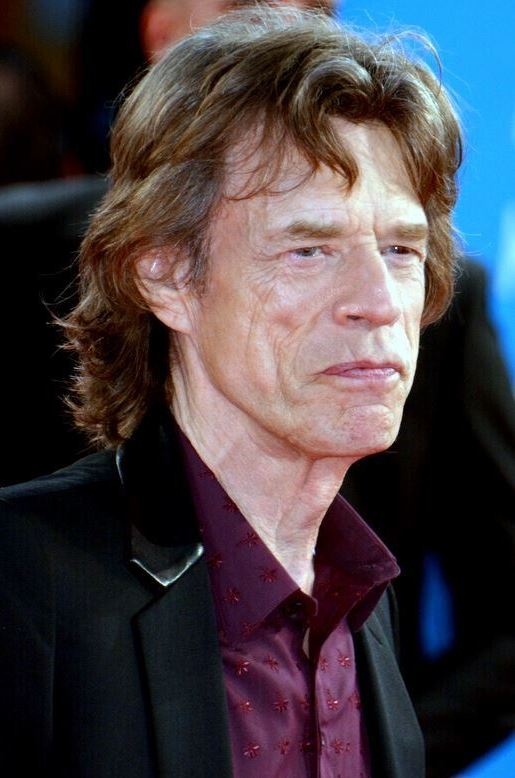
\includegraphics[width=3.5cm]{./figures/jagger.jpg}} \\
            \tiny{{\scshape Mick Jagger -} formado em economia pela LSE.}
        \end{tabular}        
        & \begin{tabular}{l}
               \parbox{0.6\linewidth}{
                \begin{itemize}
                    \item \hlight{Escassez} - recursos são limitados \bigskip
                    \NB{\href{https://youtu.be/ZUqSNbJuGOw}{you can't always get what you want} \\ \medskip Rolling Stones.}       \bigskip
                    \item O verdadeiro custo de um bem ou serviço é o valor da melhor alternativa de uso dos recursos utilizados para se adquirir esse bem - \hlight{custo de oportunidade}. \bigskip
                    \item E.g.: custo de fazer graduação em uma universidade pública?
                \end{itemize}
               }               
           \end{tabular}           
    \end{tabular}        
\end{frame}

\begin{frame}
    {Microeconomia I: postulados básicos de economia}
    \begin{itemize}
        \item Escassez $\Rightarrow$ necessidade de escolher entre alternativas possíveis \bigskip
        \item Se queremos produzir mais de um determinado bem, teremos de produzir menos de outro - \hlight{tradeoff}
    \end{itemize}
\end{frame}

\begin{frame}
    {Microeconomia I: postulados básicos de economia}
    \begin{itemize}
        \item Agentes econômicos tomam decisões visando atingir algum objetivo que têm em mente \bigskip
        \item Por que estudamos agentes individuais? Razão prática: teorias sobre comportamento individual bem estabelecidas, enquanto teorias de comportamento em grupo não é tão bem estabelecida \bigskip
        
        \item[\emoji{warning}] Note, no entanto, que decisões em grupo são fundamentais em macroeconomia e em alguns campos da micro
    \end{itemize}
\end{frame}

\begin{frame}
    {Microeconomia I: postulados básicos de economia}
    \begin{itemize}
        \item \hlight{Substituição:} agentes estão dispostos a fazer as escolhas que a escassez de recursos exige \bigskip
        \item Entre quaisquer dois bens $A$ e $B$ que desejamos, estamos dispostos a abrir mão de um pouco de $A$ para receber um pouco de $B$ \bigskip
        \item Essa substituição, normalmente, envolve pequenos incrementos dos bens - chamados de \hlight{marginais} \bigskip
        \item E.g.: o quanto investir na nossa educação?
    \end{itemize}
\end{frame}

\begin{frame}
    {Microeconomia I: postulados básicos de economia}
    \begin{tabular}{lc}
        \begin{tabular}{l}
               \parbox{0.6\linewidth}{
                \begin{itemize}
                    \item Agentes tomam suas decisões dependendo dos custos e benefícios envolvidos nessas escolhas \medskip
                    \item Quando há alterações nestes custos e benefícios, as decisões se modificam \medskip
                    
                    \NB{\emoji{warning} \hlight{Incentivos} importam!} \medskip
                    \item Podem ser colocados incentivos na economia para induzir certos tipos de decisões - aumento do combustível, pode induzir redução no uso de automóveis\medskip
                    \item Reconhecimento de que os agentes respondem a incentivos é fundamental - formuladores de política devem considerar uma mudança possível de comportamento que pode ter efeitos indesejáveis (e.g., lei seca)
                \end{itemize}
               }               
            \end{tabular}        
               & \begin{tabular}{c}
                \href{https://en.wikipedia.org/wiki/Prohibition_in_the_United_States}{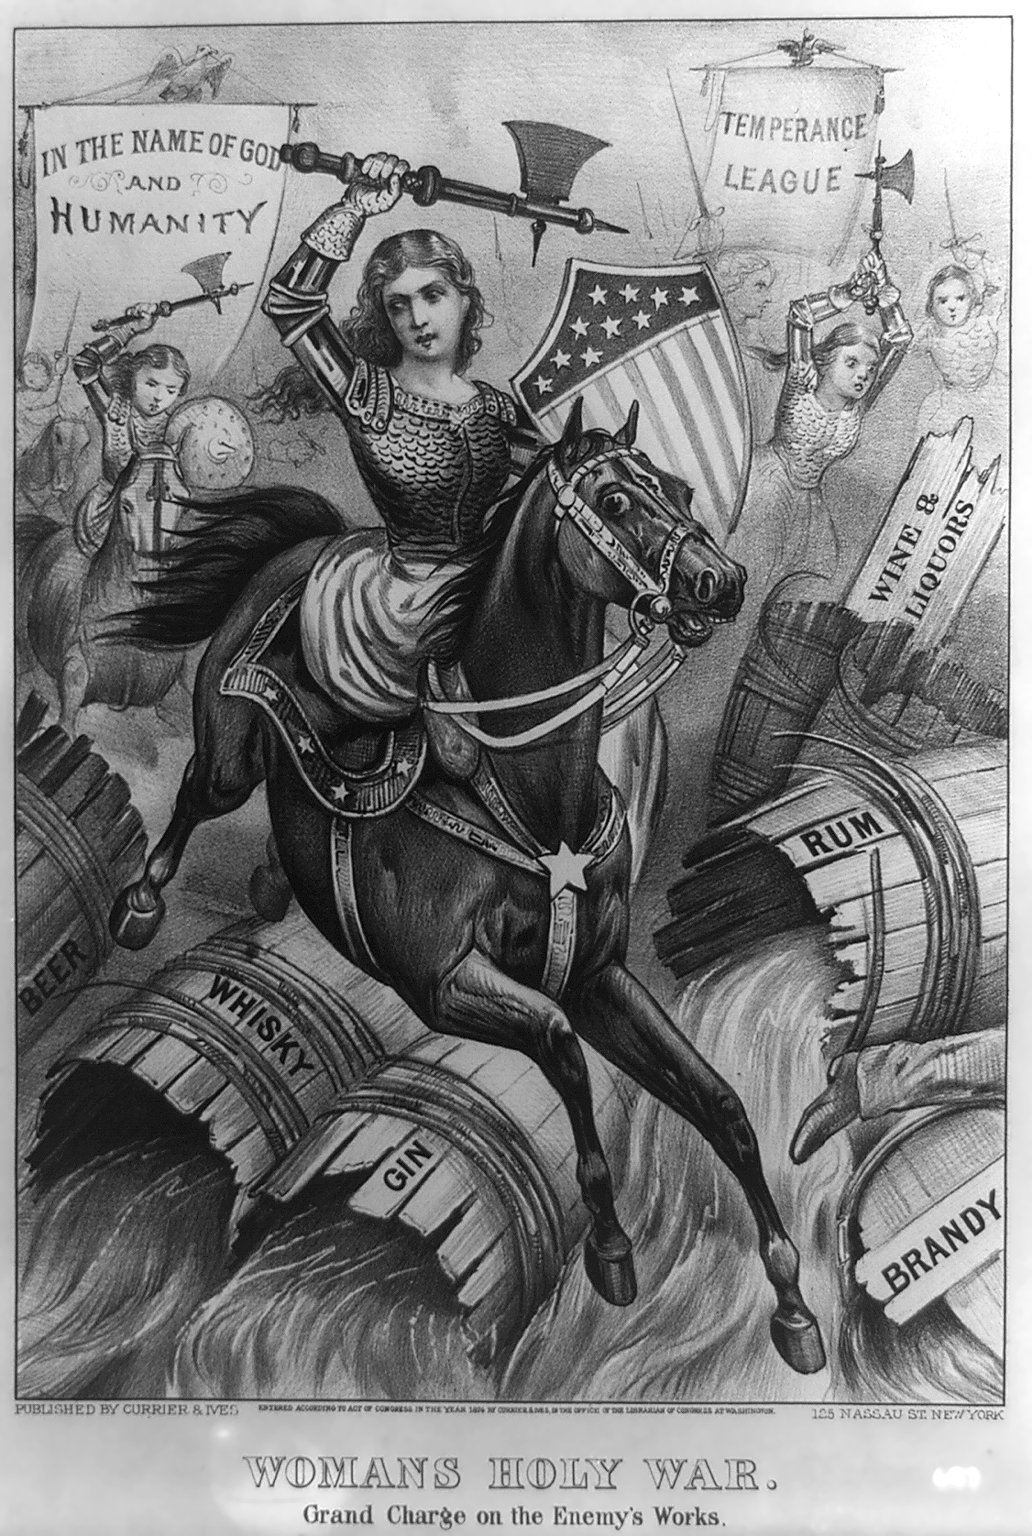
\includegraphics[width=3.5cm]{./figures/lei seca.jpg}} \\
                \tiny{{\scshape Lei seca nos EUA (1920 - 1933)}}            
           \end{tabular}           
    \end{tabular}        
\end{frame}

\begin{frame}{Microeconomia I}
    A ênfase da disciplina 23MIC1 - Microeconomia I é compreender a rationale das decisões dos agentes econômicos e o propósito do curso é fornecer uma base microeconômica sólida, que será extensivamente adotada em outras disciplinas de economia. O curso será dividido em quatro blocos:\bigskip
    \begin{enumerate}
        \item Introdução \medskip
        \item Comportamento do consumidor e demanda: teoria da preferência binária \medskip
        \item Comportamento do produtor e oferta\medskip
        \item Equilíbrio parcial de mercados perfeitamente competitivos
    \end{enumerate}
\end{frame}

\section{Ementa}
\begin{frame}{Microeconomia I: Ementa}
    \begin{center}
        \begin{minipage}{.9\textwidth}
            \NB{\hlight{Teoria do consumidor:} Restrição orçamentária. Preferências do consumidor.  Comportamento do consumidor.  Demanda individual e demanda de mercado.  Elasticidade.  Preferência revelada. Equação de Slutsky.  Escolhas sob incerteza e ativos de risco. Escolha intertemporal.  Excedente do consumidor e do produtor. \medskip \\
                \hlight{Teoria da firma:} Tecnologias de produção.  Maximização de lucros.  Minimização de custos.  Curvas de custo. Oferta da empresa e oferta de mercado.
            }
        \end{minipage}
    \end{center}

\end{frame}

\section{Objetivo}
\begin{frame}{Microeconomia I: objetivo}
    \begin{center}
        \begin{minipage}{.9\textwidth}
            \NB{A disciplina apresenta os modelos básicos referentes aos comportamentos do consumidor e do produtor, que são os blocos de construção básicos da análise microeconômica contemporânea.}
        \end{minipage}
    \end{center}
\end{frame}

\section{Formato das aulas e avaliações}
\begin{frame}{Formato das aulas e sistema de avaliação}
    \begin{itemize}
        \item A disciplina apoia-se, fundamentalmente, em livros-texto e notas de aula e será ministrada por meio de aulas expositivas.\bigskip

        \item As aulas acontecerão às:\medskip
              \begin{itemize}
                  \item Terças-feiras das 08:20 às 10:00\medskip
                  \item Quintas-feiras das 10:15 às 11:55\bigskip
              \end{itemize}

        \item A avaliação será realizada a partir dos procedimentos abaixo:\medskip
              \begin{itemize}
                  \item Atividade avaliativa I (PI): 30\%\medskip
                  \item Atividade avaliativa II (PII): 30\%\medskip
                  \item Atividade avaliativa III (PIII): 20\%\medskip
                  \item Trabalhos adicionais: 20\%
              \end{itemize}
    \end{itemize}
\end{frame}

\begin{frame}{Formato das aulas e sistema de avaliação}
    \begin{itemize}
        \item Os alunos devem ter em mente que o aprendizado e o acompanhamento do curso dependem essencialmente de seu próprio esforço.\bigskip

        \item Os tópicos do programa serão apresentados em aulas expositivas, destinadas à apresentação de conceitos, modelos e suas aplicações.\bigskip

        \item[\emoji{warning}] \hlight{Embora importantes, as aulas n\~{a}o podem jamais ser vistas como substitutas da leitura regular e cuidadosa dos textos indicados e da resolu\c{c}\~{a}o dos exerc\'{i}cios propostos.}
    \end{itemize}

\end{frame}

\section{Bibliografia}

\begin{frame}{Bibliografia \emoji{books}}
    \begin{figure}
        \centering
        \subfloat[Nicholson e Snyder (2019)\label{fig1a}]{
\includegraphics[width=0.23\textwidth]{./figures/nicholson}} \qquad
        \subfloat[Jehle e Reny (2011)\label{fig1b}]{
\includegraphics[width=0.25\textwidth]{./figures/jehle}} \qquad
        \subfloat[Mas-Colell et al. (1995)\label{fig1c}]{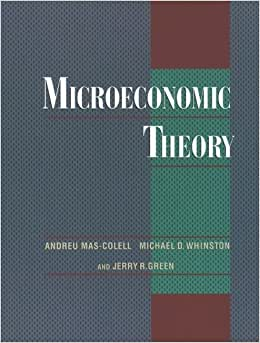
\includegraphics[width=0.25\textwidth]{./figures/colell}}
        \caption{Bibliografia do curso}
        \label{fig1}
    \end{figure}
\end{frame}

\begin{frame}{Bibliografia \emoji{books}}
    \begin{figure}
        \centering
        \subfloat[Varian (2015)\label{fig2aa}]{
\includegraphics[width=0.24\textwidth]{./figures/varian}} \qquad
        \subfloat[Pindyck e Rubinfeld (2013)\label{fig2a}]{
\includegraphics[width=0.25\textwidth]{./figures/pindyck}} \quad
        \subfloat[Vasconcellos et al. (2011)\label{fig2b}]{
\includegraphics[width=0.25\textwidth]{./figures/vasconcellos}}
        \caption{Bibliografia do curso}
        \label{fig2}
    \end{figure}
\end{frame}

\begin{frame}{Bibliografia \emoji{books}}
    \begin{itemize}
        \item JEHLE, G. A.; RENY, P. J. \emph{Advanced microeconomic theory}. 3.ed. Pearson Education Limited, 2011.\medskip
        \item MAS-COLELL, A.; WHINSTON, M.D.; GREEN, J.R. \emph{Microeconomic Theory}. New York, NY: Oxford University Press, 1995.\medskip
        \item NICHOLSON, W.; SNYDER C. \emph{Teoria microeconômica: Princípios básicos e aplicações}. Cengage Learning Brasil, 2019. Disponível em: \href{https://app.minhabiblioteca.com.br/books/9788522127030/}{app.minhabiblioteca.com.br/books/9788522127030}\medskip
        \item PINDYCK, R. S.; RUBINFELD, D. L. \emph{Microeconomia}. 8. ed. São Paulo: Pearson Education do Brasil, 2013.\medskip
        \item VARIAN, H. R. \emph{Microeconomia: uma abordagem moderna}. 9.ed. Rio de Janeiro: Elsevier, 2015. Disponível em: \href{https://app.minhabiblioteca.com.br/books/9788595155107}{app.minhabiblioteca.com.br/books/9788595155107}\medskip
        \item VASCONCELLOS, M. A. S.; OLIVEIRA, R. G.; BARBIERI, F. \emph{Manual de microeconomia}. 3.ed. São Paulo: Atlas, 2011. Disponível em: \href{https://app.minhabiblioteca.com.br/books/9788522469932/}{app.minhabiblioteca.com.br/books/9788522469932}
    \end{itemize}
\end{frame}
\end{document}